\documentclass{standalone}
\usepackage{tikz}
\begin{document}
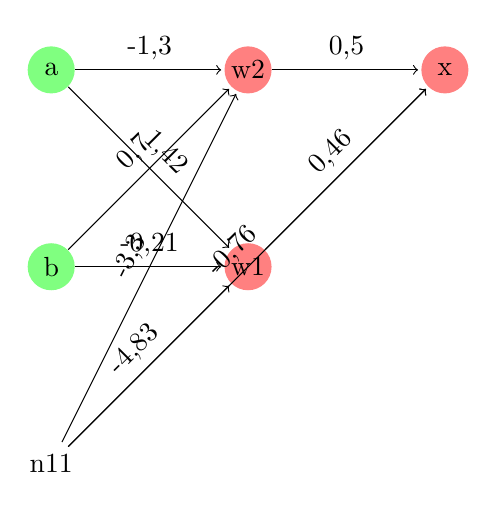
\begin{tikzpicture}[shorten >=1pt,->,draw=black!,node distance=2.5cm]
\tikzstyle{neuron}=[circle,fill=black!25,minimum size=17pt,inner sep=0pt]
\tikzstyle{constant}=[neuron, fill=white!50];
\tikzstyle{identity}=[neuron, fill=green!50];
\tikzstyle{sigmoid}=[neuron, fill=red!50];
\node [identity] (a) {a};
\node [identity,below of=a] (b) {b};
\node [constant,below of=b] (n11) {n11};
\node [sigmoid,right of=a] (w2) {w2};
\node [sigmoid,below of=w2] (w1) {w1};
\node [sigmoid,right of=w2] (x) {x};
\path[every node/.style={sloped,anchor=south,auto=false}]
(a) edge node {-1,3} (w2)
(a) edge node {1,42} (w1)
(n11) edge node {-0,76} (x)
(n11) edge node {-3,3} (w2)
(n11) edge node {-4,83} (w1)
(b) edge node {-0,21} (w1)
(b) edge node {0,7} (w2)
(w1) edge node {0,46} (x)
(w2) edge node {0,5} (x)
;\end{tikzpicture}
\end{document}